\section{Zielsetzung}
\label{sec:Zielsetzung}
In diesem Versuch wird der Photoeffekt untersucht, und die Energie der ausgelösten Elektronen durch die Gegenfeldmethode bestimmt.
\section{Theorie}
\label{sec:Theorie}

Der Photoeffekt beschreibt den Austritt von Elektronen aus einem Material, wenn es mit Licht bestrahlt wird. 
Um ihn zu erklären, muss das Korpuskelmodell von Licht verwendet werden, und nicht das Wellenmodell, welches gute Anwendung findet, sobald über eine große Anzahl von Photonen gemittelt wird. Da hier eine Wechselwirkung zwischen Licht mit Materie stattfindet, dient das Korpuskelmodell als bessere Näherung. Eine Oberfläche wird im Vakuum mit monochromatischen Licht bestrahlt. Die Photonen übertragen ihre gesamte Energie auf die Elektronen gemäß
\begin{equation}
h \nu = E_{kin} + A_k .
\end{equation}
Die Photonen besitzen die Frequenz $\nu$ und deren Energie setzt sich aus dieser und dem Plankschen Wirkungsquantum $h$ zusammen. Die Energie teilt sich in die Austrittsabeit $A_k$ aus der Kathode und die kinetische Energie der Elektronen auf. 
Damit der Photoeffekt auftritt, muss die Austrittsarbeit also kleiner sein als die Energie der Photonen, wobei somit eine Grenzfrequenz existieren muss. 
An der Gleichung ist außerdem zu erkennen, dass die kinetische Energie proportional zu der Frequenz ist.
Außerdem ist die Zahl der ausgelösten Elektronen pro Zeit- und Raumeinheit proportional zur Lichtintensität, da ein Photon höchstens mit einem Elektron wechselwirken kann.

Um die Energie der ausgelösten Elektronen zu bestimmen, wird die Gegenfeldmethode angewandt.
Eine Spannung erzeugt ein abbremsendes Feld für die Elektronen. Es erreichen also nur die Elektronen die Anode, deren Energie größer ist als $e_0 U$.
Gilt
\begin{align}
  e_0 U_g = \frac{1}{2} m_0 v_{max}^2
\end{align}
so verschwindet theoretisch der Strom. Die Geschwindigkeit $v_{max}$ ist die der schnellsten Elektronen.
Für die Energie der schnellsten Elektronen gilt dann
\begin{equation}
  h \nu = e_0 U_g  + A_k .
\end{equation}
Allerdings sinkt der Strom bei der Grenzspannung $U_g$ nicht direkt auf Null, sondern schon vorher. Dies ist in Abbildung (1) zu erkennen. 
\begin{figure}[H]
  \centering
  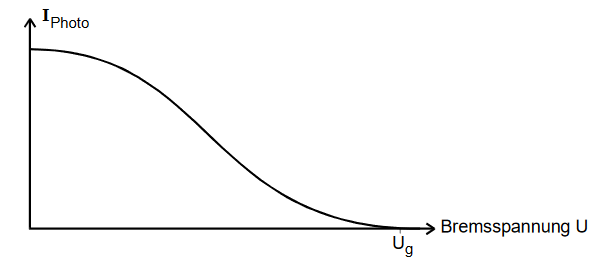
\includegraphics[height=5cm]{strom.PNG}
  \caption{Photostrom in Abhängigkeit von der Bremsspannung. \cite{kent}}
  \label{fig:kathode}
\end{figure}
Erklären lässt es sich dadurch, dass die Elektronen im Festkörper laut der Fermi-Dirac-Statistik eine Energieverteilung von $0$ bis zur Fermi-Energie $\zeta$ besitzen. Somit sind die Elektronen nicht monoenergetisch, sondern können Energien bis höchstens $h \nu - A_k$ besitzen.
Unter bestimmten Voraussetzungen, beziehungsweise als Näherung für Abbildung (1) in der Nähe von dem Wert $U_g$, besteht der Zusammenhang
\begin{align*}
  I_{Ph} \propto U^2
\end{align*}
zwischen Photostrom und Bremsspannung.
Desweiteren können Elektronen die Anode nicht erreichen, wenn die Austrittsarbeit $A_A$ des Anodenmaterials zu hoch ist. Dies liegt daran, dass die Elektronen dann gegen ein Gegenfeld anlaufen müssen, um zur Anode zu gelangen. Wird dann ein beschleunigendes Potential $U_b$ angelegt, können die Elektronen die Anode wieder erreichen und es fließt ein Photostrom, denn dann gilt
\begin{equation}
  h \nu + e_0 U_b  \geq  A_k .
\end{equation}





